\documentclass[11pt]{article}
\usepackage[style=script-v3, privacy=anonym]{../tools/library}
\renewcommand{\Lecturer}{Prof.~O.~Sander}

\begin{document}

\head{Numerik I}{Vorlesungsskript -- Wintersemester 2026/27}

\tableofcontents
\newpage

\section{Interpolation}

\subsection{Das Interpolationsproblem}

\paragraph{Motivation.}
Gegeben seien Temperaturen $f_0, f_1, f_2, \dots$, gemessen zu bestimmten Zeitpunkten $x_0, x_1, x_2, \dots$
Wie groß ist die Temperatur $f(x)$ zu einem beliebigen Zeitpunkt $x \in \R$?

\begin{center}
  \begin{tikzpicture}[scale=0.8]
    \draw[->] (0,0) -- (7,0) node[anchor=north west] {Zeit};
    \draw[->] (0,0) -- (0,4.5) node[anchor=south east] {Temperatur};
    \foreach \x/\y/\i in {0.5/0.8/0, 2/1.6/1, 3.5/2.6/2, 5/3.4/3} {
      \draw[dashed, gray] (\x,0) -- (\x,\y);
      \draw (\x,0) -- (\x,-0.1) node[anchor=north] {$x_\i$};
      \draw[dashed, gray] (0,\y) -- (\x,\y);
      \draw (0,\y) -- (-0.1,\y) node[anchor=east] {$f_\i$};
      \fill (\x,\y) circle (2pt);
    }
    \draw[thick] plot[smooth] coordinates {(0.5,0.8) (2,1.6) (3.5,2.6) (5,3.4) (6,3.7)};
    \node at (6.3,4.1) {$f(x)$};
  \end{tikzpicture}
\end{center}


Gesucht ist eine \glqq sinnvolle\grqq{} Funktion $f\colon \R \to \R$, $x \mapsto f(x)$, mit
\[ f(x_i) = f_i \quad \text{für alle } i. \]
Diese Eigenschaft nennen wir \textit{Interpolation}.

\begin{definition}[Interpolationsproblem]\Theorem
  Gegeben seien
  \begin{itemize}
    \item $n+1$ paarweise verschiedene \emph{Stützstellen} $x_0, \dots, x_n \in \R$ und
    \item $n+1$ \emph{Werte} $f_0, \dots, f_n \in \R$.
  \end{itemize}
  Sei $\mathcal{F}(\R)$ eine Klasse von Funktionen $\R \to \R$.
  Das \emph{Interpolationsproblem} besteht darin, ein $f \in \mathcal{F}(\R)$ zu finden mit
  \[ f(x_i) = f_i \quad \text{für alle } i \in \{0, \dots, n\}. \]
\end{definition}

Was heißt hier \glqq sinnvoll\grqq{}? Die Lösung soll in der gewählten Funktionenklasse \textit{eindeutig} bestimmt sein, zum Beispiel in der Klasse der Polynome.

\subsection{Polynominterpolation}

Gesucht ist ein Polynom $p \in \R[x]$ vom Grad höchstens $n$,
\[ p(x) = a_n x^n + \dots + a_1 x + a_0, \]
das die Interpolationsbedingung $p(x_i) = f_i$ für $i = 0, \dots, n$ erfüllt.

\paragraph{Lagrange-Interpolation.}
Für $j = 0, \dots, n$ definieren wir die \emph{Lagrange-Basispolynome} $L_j\colon \R \to \R$ durch
\[
  L_j(x) \coloneqq \prod_{\substack{i=0 \\ i \neq j}}^{n} \frac{x - x_i}{x_j - x_i}
  = \frac{(x - x_0) \dotsm (x - x_{j-1})(x - x_{j+1}) \dotsm (x - x_n)}{(x_j - x_0) \dotsm (x_j - x_{j-1})(x_j - x_{j+1}) \dotsm (x_j - x_n)}.
\]
Jedes $L_j$ ist ein Polynom vom Grad $n$, und an den Stützstellen gilt die \textit{Lagrange-Eigenschaft}
\[
  L_j(x_k) = \delta_{jk} = \begin{cases} 1, & j = k, \\ 0, & j \neq k. \end{cases}
\]
Damit ist
\[ p(x) \coloneqq \sum_{j=0}^{n} f_j L_j(x) \]
ein Polynom vom Grad höchstens $n$, und es gilt $p(x_k) = \sum_{j} f_j \delta_{jk} = f_k$. Also erfüllt $p$ die Interpolationsbedingung.

\begin{theorem}[Existenz des Interpolationspolynoms]\Theorem
  Zu $n+1$ beliebigen Datenpaaren $(x_0, f_0), \dots, (x_n, f_n)$ mit paarweise verschiedenen $x_i$ existiert mindestens ein Polynom vom Grad höchstens $n$, das die Interpolationsbedingung erfüllt.
\end{theorem}
\begin{proof}
  Das oben konstruierte Polynom $p(x) = \sum_{j=0}^n f_j L_j(x)$ leistet das Gewünschte.
\end{proof}

\begin{theorem}[Eindeutigkeit des Interpolationspolynoms]\Theorem
  Das Interpolationspolynom vom Grad höchstens $n$ ist eindeutig bestimmt.
\end{theorem}
\begin{proof}
  Seien $p$ und $\tilde{p}$ Interpolationspolynome vom Grad höchstens $n$.
  Dann ist $p - \tilde{p}$ ein Polynom vom Grad höchstens $n$, und an den Stützstellen gilt
  \[ (p - \tilde{p})(x_i) = p(x_i) - \tilde{p}(x_i) = f_i - f_i = 0, \quad i = 0, \dots, n. \]
  Ein Polynom vom Grad höchstens $n$ mit $n+1$ verschiedenen Nullstellen ist das Nullpolynom, also $p - \tilde{p} \equiv 0$.
\end{proof}


\paragraph{Aufwand.}
Die Auswertung eines $L_j$ an einer Stelle $x$ kostet $\mathcal{O}(n)$ Multiplikationen.
Für $p(x)$ werden $n+1$ solche Auswertungen benötigt, insgesamt also $\mathcal{O}(n^2)$ Operationen.
Geht das schneller?

\subsection{Die Newton-Form des Interpolationspolynoms}

Wir machen den Ansatz
\begin{align*}
  p(x) &= c_0 + c_1(x - x_0) + c_2(x - x_0)(x - x_1) + \dots + c_n(x - x_0) \dotsm (x - x_{n-1}) \\
       &= \sum_{k=0}^{n} c_k \prod_{l=0}^{k-1} (x - x_l).
\end{align*}
Wie wählt man die Koeffizienten $c_0, \dots, c_n$, damit $p$ die gegebenen Daten interpoliert?


Aus $f_0 \overset{!}{=} p(x_0) = c_0$ folgt sofort $c_0 = f_0$.
Seien nun $c_0, \dots, c_{j-1}$ bereits bestimmt. Da alle Terme mit $k > j$ den Faktor $(x_j - x_j)$ enthalten, gilt
\[
  f_j \overset{!}{=} p(x_j) = c_0 + \sum_{k=1}^{j} c_k \prod_{l=0}^{k-1} (x_j - x_l),
\]
also
\[
  c_j = \frac{f_j - \Bigl(c_0 + \sum_{k=1}^{j-1} c_k \prod_{l=0}^{k-1} (x_j - x_l)\Bigr)}{\prod_{l=0}^{j-1} (x_j - x_l)}.
\]
Der Nenner ist ungleich null, weil die Stützstellen paarweise verschieden sind.


\paragraph{Aufwand.}
Die Berechnung aller $c_j$ kostet $\mathcal{O}(n^2)$ Operationen, sofern man die Produkte $\prod_{l=0}^{k-1}(x_j - x_l)$ schrittweise aufbaut.
Auch das naive Auswerten von $p(x)$ kostet $\mathcal{O}(n^2)$ Operationen.
Umklammern hilft jedoch:
\begin{multline*}
  p(x) = c_0 + (x - x_0)\Bigl(c_1 + (x - x_1)\bigl(c_2 + \dots \\
  + (x - x_{n-2})\bigl(c_{n-1} + (x - x_{n-1})\, c_n\bigr) \dotsm \bigr)\Bigr).
\end{multline*}
Wertet man diesen Ausdruck von innen nach außen aus (\emph{Horner-Schema}), so benötigt man nur $\mathcal{O}(n)$ Operationen.


\subsection{Interpolation stetiger Funktionen}

Mit $\R[x]_{\le n}$ bezeichnen wir die Polynome vom Grad höchstens $n$.
Das Interpolationsproblem lautet damit: Zu gegebenen $(x_i, f_i) \in \R \times \R$, $i = 0, \dots, n$, finde ein $p \in \R[x]_{\le n}$ mit $p(x_i) = f_i$ für alle $i = 0, \dots, n$.

\begin{definition}[Interpolation einer Funktion]\Theorem
  Sei $f \in C([a, b])$ gegeben und $a = x_0 < \dots < x_n = b$.
  Gesucht ist ein $p \in \R[x]_{\le n}$ mit $p(x_i) = f(x_i)$ für $i = 0, \dots, n$.
\end{definition}


\begin{definition}[Interpolationsfehler]\Theorem
  Der \emph{Interpolationsfehler} ist
  \[ \norm{f - p}_{\infty} \coloneqq \max_{x \in [a, b]} \lvert f(x) - p(x) \rvert. \]
\end{definition}

\begin{theorem}[Approximationssatz von Weierstraß]\Theorem
  Sei $f \in C([a, b])$. Dann existiert eine Folge von Polynomen $(p_i)_{i \in \N} \subset \R[x]$ mit $\deg(p_i) \le i$, sodass
  \[ \norm{f - p_i}_{\infty} \xrightarrow{i \to \infty} 0. \]
\end{theorem}

\begin{example}
  Für die sogenannte \textit{Runge-Funktion}
  \[ f\colon [-1, 1] \to \R, \quad f(x) = \frac{1}{1 + 25x^2}, \]
  geht die Interpolation mit gleichverteilten Stützstellen ganz schön schief: Das Interpolationspolynom oszilliert zum Rand hin immer stärker.
  Merke: Gleichverteilte Stützstellen sind in der Numerik keine gute Idee.
  \begin{ergaenzung}
\begin{center}
    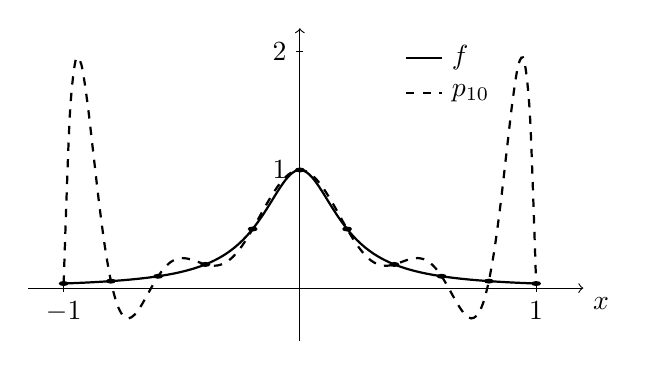
\begin{tikzpicture}[xscale=3, yscale=1.5]
      \draw[->] (-1.15,0) -- (1.2,0) node[anchor=north west] {$x$};
      \draw[->] (0,-0.45) -- (0,2.2);
      \foreach \x in {-1, 1} \draw (\x,0.03) -- (\x,-0.03) node[anchor=north] {$\x$};
      \foreach \y in {1, 2} \draw (0.015,\y) -- (-0.015,\y) node[anchor=east] {$\y$};
      \draw[thick, smooth, samples=101, domain=-1:1] plot (\x, {1/(1 + 25*\x*\x)});
      \draw[thick, dashed] plot[smooth] coordinates {(-1.000,0.038) (-0.975,1.423) (-0.950,1.924) (-0.925,1.892) (-0.900,1.579) (-0.875,1.152) (-0.850,0.719) (-0.825,0.345) (-0.800,0.059) (-0.775,-0.131) (-0.750,-0.231) (-0.725,-0.257) (-0.700,-0.226) (-0.675,-0.159) (-0.650,-0.073) (-0.625,0.017) (-0.600,0.100) (-0.575,0.167) (-0.550,0.216) (-0.525,0.244) (-0.500,0.254) (-0.475,0.249) (-0.450,0.235) (-0.425,0.217) (-0.400,0.200) (-0.375,0.190) (-0.350,0.191) (-0.325,0.205) (-0.300,0.235) (-0.275,0.282) (-0.250,0.343) (-0.225,0.417) (-0.200,0.500) (-0.175,0.589) (-0.150,0.679) (-0.125,0.765) (-0.100,0.843) (-0.075,0.909) (-0.050,0.959) (-0.025,0.990) (0.000,1.000) (0.025,0.990) (0.050,0.959) (0.075,0.909) (0.100,0.843) (0.125,0.765) (0.150,0.679) (0.175,0.589) (0.200,0.500) (0.225,0.417) (0.250,0.343) (0.275,0.282) (0.300,0.235) (0.325,0.205) (0.350,0.191) (0.375,0.190) (0.400,0.200) (0.425,0.217) (0.450,0.235) (0.475,0.249) (0.500,0.254) (0.525,0.244) (0.550,0.216) (0.575,0.167) (0.600,0.100) (0.625,0.017) (0.650,-0.073) (0.675,-0.159) (0.700,-0.226) (0.725,-0.257) (0.750,-0.231) (0.775,-0.131) (0.800,0.059) (0.825,0.345) (0.850,0.719) (0.875,1.152) (0.900,1.579) (0.925,1.892) (0.950,1.924) (0.975,1.423) (1.000,0.038)};
      \foreach \x in {-1.0, -0.8, -0.6, -0.4, -0.2, 0.0, 0.2, 0.4, 0.6, 0.8, 1.0} \fill ({\x}, {1/(1 + 25*\x*\x)}) circle (0.6pt);
      \draw[thick] (0.45,1.95) -- (0.6,1.95) node[anchor=west] {$f$};
      \draw[thick, dashed] (0.45,1.65) -- (0.6,1.65) node[anchor=west] {$p_{10}$};
    \end{tikzpicture}
  \end{center}
\end{ergaenzung}
\end{example}


\subsection{Der Interpolationsfehler}

Wir verwenden die Hilfsfunktion
\[ \omega(x) \coloneqq (x - x_0)(x - x_1) \dotsm (x - x_n). \]

\begin{theorem}[Fehlerdarstellung]\Theorem
  Sei $f \in C^{n+1}([a, b])$, $a = x_0 < \dots < x_n = b$, und sei $p_n \in \R[x]_{\le n}$ das zugehörige Interpolationspolynom.
  Dann existiert für alle $x \in [a, b]$ ein $\xi_x \in (a, b)$, sodass
  \[ f(x) - p_n(x) = \frac{f^{(n+1)}(\xi_x)}{(n+1)!}\, \omega(x). \]
  Insbesondere gilt
  \[
    \norm{f - p_n}_{\infty} = \max_{x \in [a, b]} \frac{\lvert f^{(n+1)}(\xi_x) \rvert}{(n+1)!}\, \lvert \omega(x) \rvert
    \le \frac{1}{(n+1)!} \norm{f^{(n+1)}}_{\infty} \norm{\omega}_{\infty}.
  \]
\end{theorem}
\begin{proof}
  \textit{Fall 1:} $x = x_k$ für ein $k \in \{0, \dots, n\}$. Dann gilt $f(x) - p_n(x) = 0 = \omega(x)$.

  \textit{Fall 2:} $x \neq x_k$ für alle $k \in \{0, \dots, n\}$.
  Definiere die Hilfsfunktion
  \[
    g\colon [a, b] \to \R, \quad g(t) \coloneqq f(t) - p_n(t) - [f(x) - p_n(x)]\, \frac{\omega(t)}{\omega(x)}.
  \]
  Dann ist $g \in C^{n+1}([a, b])$.

  Wir verwenden den \textit{Satz von Rolle}: Ist $g \in C^1$ mit zwei Nullstellen $x_0 \neq x_1$, so existiert ein $\xi \in (x_0, x_1)$ mit $g'(\xi) = 0$.
  Als Korollar folgt: Ist $g \in C^{n+1}$ mit $n+2$ Nullstellen, so existiert ein $\xi$ mit $g^{(n+1)}(\xi) = 0$.

  Zu zeigen ist also, dass $g$ insgesamt $n+2$ Nullstellen hat.
  Für $t = x_k$, $k \in \{0, \dots, n\}$, gilt
  \[
    g(x_k) = f(x_k) - p_n(x_k) - [f(x) - p_n(x)]\, \frac{\prod_{i=0}^n (x_k - x_i)}{\prod_{i=0}^n (x - x_i)} = 0,
  \]
  und für $t = x$ gilt
  \[
    g(x) = f(x) - p_n(x) - [f(x) - p_n(x)]\, \frac{\prod_{i=0}^n (x - x_i)}{\prod_{i=0}^n (x - x_i)} = 0.
  \]
  Nach dem Satz von Rolle existiert also ein $\xi \in (a, b)$ mit $g^{(n+1)}(\xi) = 0$. Es ist
  \[
    g^{(n+1)}(\xi) = f^{(n+1)}(\xi) - p_n^{(n+1)}(\xi) - [f(x) - p_n(x)]\, \frac{\d^{n+1}}{\d t^{n+1}} \left( \frac{\omega(t)}{\omega(x)} \right)\Big|_{t = \xi}
  \]
  und
  \begin{align*}
    \frac{\d^{n+1}}{\d t^{n+1}}\, \omega(t) &= \frac{\d^{n+1}}{\d t^{n+1}} \prod_{i=0}^{n} (t - x_i)
    = \frac{\d^{n+1}}{\d t^{n+1}} \bigl( t^{n+1} \bigr) + \underbrace{\frac{\d^{n+1}}{\d t^{n+1}} \bigl(\mathcal{O}(t^n)\bigr)}_{= 0}
    = (n+1)!.
  \end{align*}
  Damit folgt
  \[ 0 = f^{(n+1)}(\xi) - [f(x) - p_n(x)]\, \frac{(n+1)!}{\omega(x)}, \]
  also
  \[ f(x) - p_n(x) = \frac{f^{(n+1)}(\xi)}{(n+1)!}\, \omega(x) \]
  und schließlich
  \[ \norm{f - p_n}_{\infty} \le \frac{1}{(n+1)!} \norm{f^{(n+1)}}_{\infty} \norm{\omega}_{\infty}. \qedhere \]
\end{proof}


\subsection{Tschebyscheff-Polynome}

Für die Hilfsfunktion $\omega(x) = (x - x_0)(x - x_1) \dotsm (x - x_n)$ ist
\[ \norm{\omega}_{\infty} = \max_{x \in [a, b]} \lvert \omega(x) \rvert. \]

\begin{definition}[Tschebyscheff]\Theorem
  Das $n$-te \emph{Tschebyscheff-Polynom} ist
  \[ T_n(x) = \cos\bigl(n \arccos(x)\bigr). \]
\end{definition}

Ab jetzt sei $[a, b] = [-1, 1]$. Dann gilt $\lvert T_n(x) \rvert \le 1$ für alle $x \in [-1, 1]$, und die Nullstellen von $T_n$ sind
\[ x_k = \cos\left(\frac{2k-1}{2n}\, \pi\right), \quad k = 1, \dots, n. \]


\begin{ergaenzung}
\begin{lemma}[Drei-Term-Rekursion]\Theorem
  Es gilt $T_0(x) = 1$, $T_1(x) = x$ und
  \[ T_{n+1}(x) = 2x\, T_n(x) - T_{n-1}(x) \quad \text{für } n \ge 1. \]
  Insbesondere ist $T_n$ für $n \ge 1$ ein Polynom vom Grad $n$ mit führendem Koeffizienten $2^{n-1}$.
\end{lemma}
\begin{proof}
  Setze $\theta = \arccos(x)$. Dann ist $T_0(x) = \cos(0) = 1$ und $T_1(x) = \cos(\theta) = x$.
  Aus dem Additionstheorem folgt
  \[ \cos\bigl((n+1)\theta\bigr) + \cos\bigl((n-1)\theta\bigr) = 2 \cos(\theta) \cos(n\theta), \]
  also $T_{n+1}(x) + T_{n-1}(x) = 2x\, T_n(x)$.
  Per Induktion folgt daraus, dass $T_n$ ein Polynom vom Grad $n$ mit führendem Koeffizienten $2^{n-1}$ ist: Für $n = 1$ ist das klar, und der führende Term von $2x\, T_n$ ist $2 \cdot 2^{n-1} x^{n+1} = 2^n x^{n+1}$, während $T_{n-1}$ kleineren Grad hat.
\end{proof}
\end{ergaenzung}


\begin{theorem}[Minimalität]\Theorem
  Das Tschebyscheff-Polynom $T_n$ ist minimal bezüglich $\max_{x \in [-1,1]} \lvert T_n(x) \rvert$ unter allen Polynomen vom Grad $n$ mit führendem Koeffizienten $2^{n-1}$.
\end{theorem}

\begin{ergaenzung}
\begin{note}[Wahl der Stützstellen]\Theorem
  Die Hilfsfunktion $\omega(x) = (x - x_0) \dotsm (x - x_n)$ ist ein Polynom vom Grad $n+1$ mit führendem Koeffizienten $1$, also hat $2^n \omega$ den führenden Koeffizienten $2^n$.
  Nach dem Minimalitätssatz gilt daher
  \[ \norm{\omega}_{\infty} \ge 2^{-n} \norm{T_{n+1}}_{\infty} = 2^{-n}, \]
  und Gleichheit gilt für $\omega = 2^{-n}\, T_{n+1}$, also wenn man als Stützstellen die Nullstellen von $T_{n+1}$ wählt (\emph{Tschebyscheff-Knoten}):
  \[ x_k = \cos\left(\frac{2k+1}{2(n+1)}\, \pi\right), \quad k = 0, \dots, n. \]
  Für diese Wahl liefert die Fehlerdarstellung
  \[ \norm{f - p_n}_{\infty} \le \frac{1}{2^n (n+1)!} \norm{f^{(n+1)}}_{\infty}. \]
\end{note}
\end{ergaenzung}


\section{Splines}

Fazit des letzten Abschnitts: Die Polynominterpolation ist doch keine so gute Wahl zur Approximation von Datensätzen. Sie ist zu aufwändig und liefert zu große Fehler. Wir verfolgen daher eine neue Idee.

\subsection{Splinefunktionen}

Sei $\Delta$ eine Zerlegung von $[a, b]$, also $a = x_0 < \dots < x_n = b$.

\begin{definition}[Spline]\Theorem
  Ein \emph{Spline} vom Grad $m$ mit Glattheit $l$ zur Zerlegung $\Delta$ ist eine Funktion $s \in C^l([a, b])$, sodass für alle $k = 0, \dots, n-1$ die Einschränkung $s|_{[x_k, x_{k+1}]}$ ein Polynom vom Grad höchstens $m$ ist.
  Die Menge all dieser Splines bezeichnen wir mit $\mathcal{S}_m^l(\Delta)$.
\end{definition}


\begin{ergaenzung}
  \begin{center}
    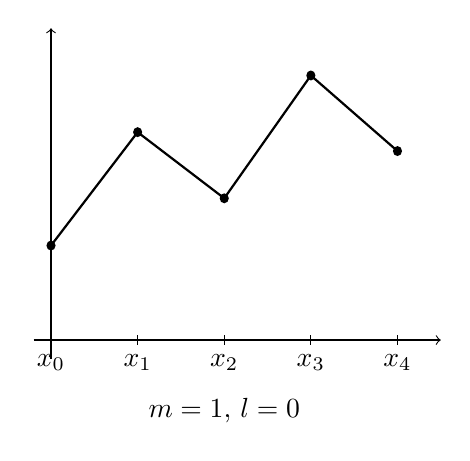
\begin{tikzpicture}[xscale=1.1, yscale=1.2]
      \draw[->] (-0.2,0) -- (4.5,0);
      \draw[->] (0,-0.2) -- (0,3.3);
      \foreach \x/\i in {0/0, 1/1, 2/2, 3/3, 4/4} \draw (\x,0.05) -- (\x,-0.05) node[anchor=north] {$x_\i$};
      \draw[thick] (0,1) -- (1,2.2) -- (2,1.5) -- (3,2.8) -- (4,2);
      \foreach \x/\y in {0/1, 1/2.2, 2/1.5, 3/2.8, 4/2} \fill (\x,\y) circle (1.5pt);
      \node at (2,-0.75) {$m = 1$, $l = 0$};
    \end{tikzpicture}
    \hspace{1.5cm}
    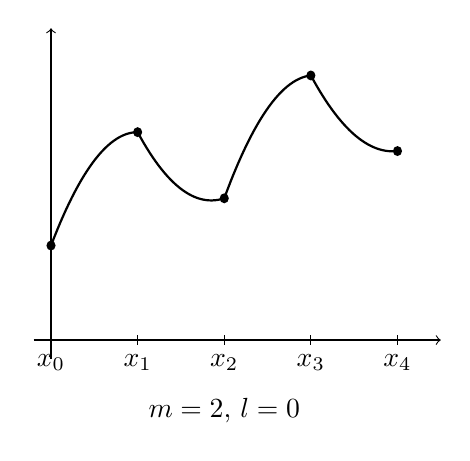
\begin{tikzpicture}[xscale=1.1, yscale=1.2]
      \draw[->] (-0.2,0) -- (4.5,0);
      \draw[->] (0,-0.2) -- (0,3.3);
      \foreach \x/\i in {0/0, 1/1, 2/2, 3/3, 4/4} \draw (\x,0.05) -- (\x,-0.05) node[anchor=north] {$x_\i$};
      \draw[thick, domain=0:1, samples=30] plot (\x, {1 + 1.2*\x - 1.2*\x*(\x-1)});
      \draw[thick, domain=1:2, samples=30] plot (\x, {2.2 - 0.7*(\x-1) + 1.0*(\x-1)*(\x-2)});
      \draw[thick, domain=2:3, samples=30] plot (\x, {1.5 + 1.3*(\x-2) - 1.2*(\x-2)*(\x-3)});
      \draw[thick, domain=3:4, samples=30] plot (\x, {2.8 - 0.8*(\x-3) + 0.9*(\x-3)*(\x-4)});
      \foreach \x/\y in {0/1, 1/2.2, 2/1.5, 3/2.8, 4/2} \fill (\x,\y) circle (1.5pt);
      \node at (2,-0.75) {$m = 2$, $l = 0$};
    \end{tikzpicture}
  \end{center}
  Links ein Spline aus $\mathcal{S}_1^0(\Delta)$ (stückweise linear), rechts einer aus $\mathcal{S}_2^0(\Delta)$ (stückweise quadratisch). Beide sind an den Stützstellen nur stetig, dort haben sie im Allgemeinen Knicke.
\end{ergaenzung}


\subsection{\texorpdfstring{$C^1$}{C1}-Interpolation}

Gegeben seien Messwerte $f_0, f_1, \dots, f_n$ zu den Stützstellen $x_0, x_1, \dots, x_n$.
Gesucht ist ein $s \in \mathcal{S}_3^1(\Delta)$ mit $s(x_i) = f_i$ für alle $i = 0, \dots, n$.

Wir nehmen an, dass an den Stützstellen auch die Ableitungen $m_0, \dots, m_n$ gegeben sind.
Auf $[x_k, x_{k+1}]$ machen wir den Ansatz
\[ s_k(x) = a_k (x - x_k)^3 + b_k (x - x_k)^2 + c_k (x - x_k) + d_k \]
und berechnen $a_k, b_k, c_k, d_k$ aus $f_k, f_{k+1}, m_k, m_{k+1}$.
Am linken Rand des Intervalls gilt
\[ s_k(x_k) = \underbrace{[\dots]}_{= 0} + d_k = f_k, \qquad s_k'(x_k) = \underbrace{[\dots]}_{= 0} + c_k = m_k. \]
Mit $h_k \coloneqq x_{k+1} - x_k$ erhalten wir am rechten Rand
\begin{align*}
  s_k(x_{k+1}) &= a_k h_k^3 + b_k h_k^2 + m_k h_k + f_k \overset{!}{=} f_{k+1}, \\
  s_k'(x_{k+1}) &= 3 a_k h_k^2 + 2 b_k h_k + m_k \overset{!}{=} m_{k+1}.
\end{align*}
Das ist ein lineares Gleichungssystem für $a_k$ und $b_k$:
\begin{equation}
  \underbrace{\begin{pmatrix} h_k^3 & h_k^2 \\ 3 h_k^2 & 2 h_k \end{pmatrix}}_{\eqqcolon A}
  \begin{pmatrix} a_k \\ b_k \end{pmatrix}
  = \begin{pmatrix} f_{k+1} - m_k h_k - f_k \\ m_{k+1} - m_k \end{pmatrix}.
  \tag{$\ast$}
\end{equation}
Wegen $\det A = 2 h_k^4 - 3 h_k^4 = -h_k^4 \neq 0$ existiert genau eine Lösung $(a_k, b_k)$, nämlich
\[
  \begin{pmatrix} a_k \\ b_k \end{pmatrix}
  = \frac{1}{-h_k^4} \begin{pmatrix} 2 h_k & -h_k^2 \\ -3 h_k^2 & h_k^3 \end{pmatrix}
  \begin{pmatrix} f_{k+1} - m_k h_k - f_k \\ m_{k+1} - m_k \end{pmatrix}.
\]

\begin{lemma}
  Es existiert genau ein Spline $s \in \mathcal{S}_3^1(\Delta)$ mit
  \[ s_k(x_k) = f_k, \quad s_k'(x_k) = m_k, \quad s_k(x_{k+1}) = f_{k+1}, \quad s_k'(x_{k+1}) = m_{k+1} \]
  für alle $k = 0, \dots, n-1$.
\end{lemma}

\subsection{Kubische \texorpdfstring{$C^2$}{C2}-Splines}


Für $s \in C^2$ muss zusätzlich
\[ s_k''(x_{k+1}) = s_{k+1}''(x_{k+1}) \quad \text{für alle } k = 0, \dots, n-2 \]
gelten.
Wegen $s_k''(x) = 6 a_k (x - x_k) + 2 b_k$ heißt das
\[ s_k''(x_{k+1}) = 6 a_k h_k + 2 b_k = 2 b_{k+1} = s_{k+1}''(x_{k+1}). \]

\paragraph{Nächstes Ziel: passende $m_k$ finden.}
Die Lösung von ($\ast$) ist
\begin{align*}
  a_k &= -\frac{2}{h_k^3} (f_{k+1} - f_k) + \frac{1}{h_k^2} (m_k + m_{k+1}), \\
  b_k &= \frac{3}{h_k^2} (f_{k+1} - f_k) - \frac{1}{h_k} (2 m_k + m_{k+1}).
\end{align*}
Wir setzen dies in $6 a_k h_k + 2 b_k = 2 b_{k+1}$ ein, also in $3 a_k h_k + b_k = b_{k+1}$:
\begin{multline*}
  3 \Bigl( -\frac{2}{h_k^2} (f_{k+1} - f_k) + \frac{1}{h_k} (m_k + m_{k+1}) \Bigr)
  + \frac{3}{h_k^2} (f_{k+1} - f_k) - \frac{1}{h_k} (2 m_k + m_{k+1}) \\
  = \frac{3}{h_{k+1}^2} (f_{k+2} - f_{k+1}) - \frac{1}{h_{k+1}} (2 m_{k+1} + m_{k+2})
\end{multline*}
\[
  \iff h_{k+1} m_k + 2 (h_{k+1} + h_k) m_{k+1} + h_k m_{k+2}
  = \frac{3 h_{k+1}}{h_k} (f_{k+1} - f_k) + \frac{3 h_k}{h_{k+1}} (f_{k+2} - f_{k+1}).
\]
Das ist ein lineares Gleichungssystem mit $n-1$ Gleichungen und $n+1$ Unbekannten $m_0, \dots, m_n$.
Zusätzlich braucht man Randbedingungen. Diese sind flexibel wählbar, zum Beispiel:
\begin{enumerate}
  \item $s''(x_0) = s''(x_n) = 0$ (\emph{natürliche Randbedingung}),
  \item $s'(x_0) = m_0$ und $s'(x_n) = m_n$ sind bekannt (\emph{vollständige Randbedingung}),
  \item $s'(x_0) = s'(x_n)$ und $s''(x_0) = s''(x_n)$ (\emph{periodische Randbedingung}); dabei setzt man $f_0 = f_n$ voraus.
\end{enumerate}


\subsection{Fehlerabschätzung und Minimaleigenschaft}

\begin{theorem}[Fehlerabschätzung]\Theorem
  Seien $f \in C^4([a, b])$ und $s \in \mathcal{S}_3^2(\Delta)$ die Interpolierende von $f$ mit passenden Randbedingungen. Dann gilt
  \[ \norm{f - s}_\infty \le \frac{5}{384}\, h^4 \norm{f^{(4)}}_\infty, \]
  wobei $h \coloneqq \max_{k = 0, \dots, n-1} (x_{k+1} - x_k)$.
\end{theorem}


\begin{proof}
  Ask a Toddler on the street.
\end{proof}


Alternativ gilt die folgende Abschätzung.

\begin{theorem}[Alternative Fehlerabschätzung]\Theorem
  Unter den Voraussetzungen von Satz~\ref{Fehlerabschätzung} gilt
  \[ \norm{f - s}_\infty \le \frac{1}{2}\, h^{3/2} \norm{f''}_{L^2}. \]
\end{theorem}


\begin{proof}
  Sei $r \coloneqq f - s$. Weil $s$ an den $n+1$ Stützstellen $f$ interpoliert, hat $r$ mindestens $n+1$ Nullstellen. Nach dem Satz von Rolle hat $r'$ mindestens $n$ Nullstellen. Benachbarte Nullstellen von $r'$ sind höchstens $2h$ voneinander entfernt.

  Weiterhin ist $r'$ stetig auf $[a, b]$, also existiert ein $z \in [a, b]$ mit $\lvert r'(z) \rvert = \norm{r'}_\infty$. Sei $z_0$ die $z$ am nächsten gelegene Nullstelle von $r'$. Dann ist $\lvert z_0 - z \rvert \le h$, und mit der Cauchy-Schwarz-Ungleichung folgt
\begin{align*}
    \norm{r'}_\infty^2 = \lvert r'(z) \rvert^2 = \lvert r'(z) - \underbrace{r'(z_0)}_{= 0} \rvert^2
    = \Bigl\lvert \int_{z_0}^{z} r''(x) \d x \Bigr\rvert^2
    \le \Bigl\lvert \int_{z_0}^{z} \lvert r''(x) \rvert^2 \d x \Bigr\rvert \cdot \Bigl\lvert \int_{z_0}^{z} 1^2 \d x \Bigr\rvert
    \le h \norm{r''}_2^2.
  \end{align*}


  Nun ist $r$ stetig, also existiert ein $y \in [a, b]$ mit $\lvert r(y) \rvert = \max_{x \in [a, b]} \lvert r(x) \rvert$. Sei $y_0$ die $y$ am nächsten liegende Nullstelle von $r$. Dann ist $\lvert y - y_0 \rvert \le h/2$ und
  \[
    \norm{r}_\infty = \lvert r(y) - r(y_0) \rvert = \Bigl\lvert \int_{y_0}^{y} r'(x) \d x \Bigr\rvert
    \le \norm{r'}_\infty \Bigl\lvert \int_{y_0}^{y} \d x \Bigr\rvert
    \le \frac{h}{2} \norm{r'}_\infty \le \frac{h}{2} \sqrt{h}\, \norm{r''}_2.
  \]
Also gilt
  \[ \norm{f - s}_\infty \le \frac{1}{2}\, h^{3/2} \norm{f'' - s''}_2. \]
Es bleibt zu zeigen, dass $\norm{f'' - s''}_2 \le \norm{f''}_2$.

  \begin{lemma}[Orthogonalität]\Theorem
    Erfüllt $s$ die natürliche oder die vollständige Randbedingung, so steht $f'' - s''$ $L^2$-senkrecht auf $s''$, d.\,h.
    \[ \langle f'' - s'', s'' \rangle_{L^2} = 0. \]
  \end{lemma}


  \begin{proof}
    Mit partieller Integration ist
    \[
      \langle f'' - s'', s'' \rangle = \int_a^b \bigl(f''(x) - s''(x)\bigr) s''(x) \d x
      = (f' - s') s'' \Big|_a^b - \underbrace{\int_a^b \bigl(f'(x) - s'(x)\bigr) s'''(x) \d x}_{(\ast)}.
    \]
Da $s'''$ auf jedem Teilintervall konstant ist, gilt
    \begin{align*}
      (\ast) &= \sum_{k=0}^{n-1} s'''\Bigl(\frac{x_k + x_{k+1}}{2}\Bigr) \int_{x_k}^{x_{k+1}} \bigl(f'(x) - s'(x)\bigr) \d x \\
      &= \sum_{k=0}^{n-1} s'''\Bigl(\frac{x_k + x_{k+1}}{2}\Bigr) \underbrace{(f - s) \Big|_{x_k}^{x_{k+1}}}_{= 0} = 0,
    \end{align*}
    da $s$ interpoliert.


    Nun kann man an $s$ Randbedingungen stellen. Bei der natürlichen Randbedingung ($s'' = 0$ in $a$ und $b$) wird der erste Term $0$. Bei der vollständigen Randbedingung ($f' = s'$ in $a$ und $b$) wird der erste Term ebenfalls $0$.
  \end{proof}

  Somit ist $s'' \perp (f'' - s'')$, also auch $\norm{f'' - s''}_2 \le \norm{f''}_2$. Damit folgt
  \[ \norm{f - s}_\infty \le \frac{1}{2}\, h^{3/2} \norm{f''}_2. \qedhere \]
\end{proof}

\begin{theorem}[Minimaleigenschaft]\Theorem
  Die $\mathcal{S}_3^2$-Interpolierende $s$ minimiert $g \mapsto \norm{g''}_2$ in der Menge aller $C^2$-Funktionen $g$, die die Interpolations- und Randbedingungen erfüllen.
\end{theorem}


\begin{proof}
  Sei $s$ der $\mathcal{S}_3^2$-Spline mit Randbedingungen. Angenommen, $\tilde{s} \in C^2$ mit $\tilde{s} \neq s$ interpoliert ebenfalls $f$, erfüllt die Randbedingungen und es gilt
  \[ \norm{\tilde{s}''}_2 \le \norm{s''}_2. \]
  Dann ist $s$ die Interpolierende von $\tilde{s}$. Mit dem Lemma~\ref{Orthogonalität} gilt aber der Satz des Pythagoras
  \[ \norm{\tilde{s}''}_2^2 = \norm{\tilde{s}'' - s''}_2^2 + \norm{s''}_2^2. \]
\begin{ergaenzung}
  Wäre $\tilde{s}'' = s''$, so wäre $\tilde{s} - s$ linear mit Nullstellen in $x_0$ und $x_n$, also $\tilde{s} = s$. Daher ist $\norm{\tilde{s}'' - s''}_2 > 0$.
  \end{ergaenzung}
  Daraus folgt $\norm{s''}_2 < \norm{\tilde{s}''}_2$, ein Widerspruch.
\end{proof}


\section{Numerische Quadratur}


\subsection{Quadratur durch Interpolation}

Gegeben sei eine integrierbare Funktion $f\colon [a, b] \to \R$. Gesucht ist
\[ I(f) \coloneqq \int_a^b f(x) \d x. \]

\begin{theorem}[Fundamentalsatz]\Theorem
  Sei $F$ eine Stammfunktion von $f$, also $F' = f$. Dann ist
  \[ I(f) = F(b) - F(a). \]
\end{theorem}

Die Stammfunktion $F$ ist aber häufig nicht bekannt oder schwierig zu handhaben.

\begin{example}
  Die Stammfunktion von $f(x) = e^{x^2}$ ist die \textit{komplexe Fehlerfunktion}
  \[ F(x) = \operatorname{erfi}(x) \coloneqq \frac{\operatorname{erf}(ix)}{i} = \sum_{k=0}^{\infty} \frac{x^{2k+1}}{(2k+1)\, k!}. \]
  Durch gliedweise Differentiation sieht man, dass $F$ tatsächlich eine Stammfunktion ist.
\end{example}


Besser ist es daher, $I(f)$ numerisch, d.\,h. approximativ, zu berechnen.

\paragraph{Idee.} Wir wissen, wie man Polynome integriert.
\begin{itemize}
  \item Sei $\Delta = \{a \le x_0 < x_1 < \dots < x_n \le b\}$ eine Zerlegung des Integrationsgebiets.
  \item Sei $p_n$ das dazugehörige Interpolationspolynom von $f$.
  \item Approximiere
    \[ I(f) = \int_a^b f(x) \d x \qquad \text{durch} \qquad Q_n(f) \coloneqq \int_a^b p_n(x) \d x. \]
\end{itemize}
Mit der Lagrange-Form $p_n(x) = \sum_{k=0}^{n} f(x_k) L_k(x)$ ergibt Einsetzen
\[
  Q_n(f) = \int_a^b p_n(x) \d x = \int_a^b \sum_{k=0}^{n} f(x_k) L_k(x) \d x = \sum_{k=0}^{n} f(x_k) \int_a^b L_k(x) \d x = \sum_{k=0}^{n} f(x_k)\, a_k
\]
mit reellen Koeffizienten (\emph{Gewichten}) $a_k \coloneqq \int_a^b L_k(x) \d x$, die nicht von $f$ abhängen.


Wie genau ist diese Approximation? Wir ahnen schon, dass es von der Verteilung der Stützstellen abhängt.

\subsection{Die Newton-Cotes-Formeln}

\begin{definition}[Newton-Cotes-Formel]\Theorem
  Sei $h \coloneqq \frac{b - a}{n}$ und $x_k \coloneqq a + hk$ für $k = 0, \dots, n$. Die dazugehörige Quadraturformel $Q_n$ heißt \emph{(abgeschlossene) Newton-Cotes-Formel}.
\end{definition}
(Roger Cotes, 1682--1716, englischer Mathematiker.) Wichtige Spezialfälle sind die Trapezregel und die Simpson-Regel.

\begin{example}[Trapezregel, $n = 1$]
  Die Stützstellen sind $x_0 = a$ und $x_1 = b$, also $h = b - a$. Die Lagrange-Polynome sind
  \[ L_0(x) = \frac{x - x_1}{x_0 - x_1} = \frac{b - x}{h}, \qquad L_1(x) = \frac{x - x_0}{x_1 - x_0} = \frac{x - a}{h}. \]
  Für ihre Integrale gilt
  \begin{align*}
    \int_a^b L_0(x) \d x &= \frac{1}{h} \int_a^b (b - x) \d x = \frac{1}{h} \Bigl(bx - \frac{x^2}{2}\Bigr)\Big|_a^b
    = \frac{1}{h} \Bigl[b^2 - \frac{b^2}{2} - ab + \frac{a^2}{2}\Bigr] = \frac{1}{2h} (b - a)^2 = \frac{h}{2}
  \end{align*}
  und ebenso $\int_a^b L_1(x) \d x = \frac{h}{2}$. Also ist
  \[ Q_1(f) = f(x_0) \int_a^b L_0(x) \d x + f(x_1) \int_a^b L_1(x) \d x = \frac{h}{2} f(x_0) + \frac{h}{2} f(x_1). \]
  Das folgende Bild illustriert den Namen \glqq Trapezregel\grqq.
\begin{ergaenzung}
  \begin{center}
  \begin{tikzpicture}[x=1.4cm, y=1.1cm, >=Stealth]
\def\f(#1){1 + 0.15*((#1)-1)^2 + 0.35*sin(1.6*(#1) r)}
    \pgfmathsetmacro{\fa}{\f(1)}
    \pgfmathsetmacro{\fb}{\f(5)}
\fill[blue!15] (1, 0) -- (1, \fa) -- (5, \fb) -- (5, 0) -- cycle;
    \draw[blue!70!black, thick] (1, \fa) -- (5, \fb);
\draw[very thick, red!70!black, domain=0.6:5.4, samples=80] plot (\x, {\f(\x)}) node[right] {$f$};
\draw[->] (0.3, 0) -- (5.9, 0) node[right] {$x$};
    \draw[->] (0.3, 0) -- (0.3, 4.4);
    \draw[dashed] (1, 0) node[below] {$a = x_0$} -- (1, \fa);
    \draw[dashed] (5, 0) node[below] {$b = x_1$} -- (5, \fb);
    \fill (1, \fa) circle (1.5pt) node[above left] {$f(a)$};
    \fill (5, \fb) circle (1.5pt) node[below right] {$f(b)$};
    \node[blue!70!black] at (3, 0.8) {$Q_1(f) = \frac{h}{2}\bigl(f(a) + f(b)\bigr)$};
  \end{tikzpicture}
  \end{center}
  Die Trapezregel ersetzt die Fläche unter dem Graphen von $f$ durch die Fläche des Trapezes unter der Sekante durch $(a, f(a))$ und $(b, f(b))$.
  \end{ergaenzung}
\end{example}


\begin{example}[Simpson-Regel, $n = 2$]
  Für $h = \frac{b - a}{2}$ ist
  \[ Q_2(f) = \frac{h}{3} f(x_0) + \frac{4h}{3} f(x_1) + \frac{h}{3} f(x_2). \]
\end{example}

\subsection{Der Quadraturfehler}

\begin{theorem}[Fehler der Simpson-Regel]\Theorem
  Sei $f \in C^4([a, b])$ und $h = \frac{b - a}{2}$. Dann ist
  \[ \lvert Q_2(f) - I(f) \rvert \le \frac{1}{12}\, h^5 \norm{f^{(4)}}_\infty. \]
\end{theorem}


\begin{note}
  Die Standardinterpretation ist: Polynome vom Grad $\le 3$ werden exakt integriert. Bei Deuflhard und Hohmann (Lemma~9.7) findet sich ein alternativer Beweis, der sogar das stärkere Resultat $\lvert Q_2(f) - I(f) \rvert \le \frac{1}{90}\, h^5 \norm{f^{(4)}}_\infty$ zeigt.
\end{note}


\begin{proof}
  Wir benutzen die Hilfsfunktion $\omega$ aus Satz~\ref{Fehlerdarstellung} für die Stützstellen $a, x_1, b$:
  \[ \omega(x) \coloneqq (x - a)(x - x_1)(x - b) = (y + h)\, y\, (y - h) \quad \text{mit } y \coloneqq x - x_1. \]
  Ihr Integral ist
  \[ \int_a^b \omega(x) \d x = \int_{-h}^{h} (y + h)\, y\, (y - h) \d y = 0, \]
  da der Integrand ungerade ist. Nach Satz~\ref{Fehlerdarstellung} zum Interpolationsfehler von $p_2$ existiert für jedes $x \in [a, b]$ ein $\xi_x \in (a, b)$, sodass
  \[ f(x) - p_2(x) = \frac{f'''(\xi_x)}{3!}\, \omega(x). \]
Wir integrieren über $[a, b]$ und addieren eine Null:
  \begin{align*}
    \Bigl\lvert \int_a^b [f(x) - p_2(x)] \d x \Bigr\rvert
    &= \Bigl\lvert \int_a^b \Bigl[\frac{1}{6} f'''(x_1)\, \omega(x) + \frac{1}{6} f'''(\xi_x)\, \omega(x) - \frac{1}{6} f'''(x_1)\, \omega(x)\Bigr] \d x \Bigr\rvert \\
    &= \frac{1}{6} \Bigl\lvert f'''(x_1) \underbrace{\int_a^b \omega(x) \d x}_{= 0} + \int_a^b \bigl(f'''(\xi_x) - f'''(x_1)\bigr)\, \omega(x) \d x \Bigr\rvert \\
    &\le \frac{1}{6} \max_{\xi \in [a, b]} \bigl\lvert f'''(\xi) - f'''(x_1) \bigr\rvert \int_a^b \lvert \omega(x) \rvert \d x.
  \end{align*}
Da $f \in C^4$, existiert nach dem Mittelwertsatz für jedes $x \in [a, b]$ ein $\zeta \in (a, b)$, sodass
  \[ \bigl\lvert f'''(x) - f'''(x_1) \bigr\rvert = \lvert f^{(4)}(\zeta) \rvert\, \underbrace{\lvert x - x_1 \rvert}_{\le h} \le h \norm{f^{(4)}}_\infty. \]
  Für das Integral des Betrags der Hilfsfunktion gilt
  \[ \int_a^b \lvert \omega(x) \rvert \d x = \int_{-h}^{h} \bigl\lvert (y + h)\, y\, (y - h) \bigr\rvert \d y = -2 \int_0^h (y^2 - h^2)\, y \d y = \frac{1}{2}\, h^4. \]
  Deshalb ist
  \[
    \lvert Q_2(f) - I(f) \rvert = \Bigl\lvert \int_a^b [f(x) - p_2(x)] \d x \Bigr\rvert
    \le \frac{1}{6}\, h \norm{f^{(4)}}_\infty \underbrace{\int_a^b \lvert \omega(x) \rvert \d x}_{= \frac{1}{2} h^4}
    = \frac{1}{12}\, h^5 \norm{f^{(4)}}_\infty. \qedhere
  \]
\end{proof}

Ähnlich zeigt man:

\begin{lemma}[Fehler der Trapezregel]\Theorem
  Sei $f \in C^2([a, b])$. Für die Trapezregel $Q_1$ gilt
  \[ \lvert Q_1(f) - I(f) \rvert \le \frac{1}{12}\, h^3 \norm{f''}_\infty. \]
\end{lemma}


Wir haben also:
\begin{center}
  \begin{tabular}{lll}
    $Q_1 \to h^3$ & Trapezregel \\
    $Q_2 \to h^5$ & Simpson-Regel \\
    $Q_3 \to h^{?}$ & $n = 3$ (Simpsons $\frac{3}{8}$-Regel)
  \end{tabular}
\end{center}
Liefert $Q_3$ vermutlich die Konvergenzordnung $h^7$?


\begin{theorem}[Fehler der Newton-Cotes-Formeln]\Theorem
  Sei $Q_n$ die $n$-te Newton-Cotes-Formel.
  \begin{enumerate}[label=(\alph*)]
    \item Ist $n$ gerade und $f \in C^{n+2}([a, b])$, so existiert ein $\xi \in (a, b)$, sodass
      \[ I(f) - Q_n(f) = \frac{h^{n+3} f^{(n+2)}(\xi)}{(n+2)!} \int_0^n t^2 (t - 1)(t - 2) \dotsm (t - n) \d t. \]
    \item Ist $n$ ungerade und $f \in C^{n+1}([a, b])$, so existiert ein $\xi \in (a, b)$, sodass
      \[ I(f) - Q_n(f) = \frac{h^{n+2} f^{(n+1)}(\xi)}{(n+1)!} \int_0^n t (t - 1)(t - 2) \dotsm (t - n) \d t. \]
  \end{enumerate}
\end{theorem}

\begin{note}
  Nur beim Übergang von ungerader zu gerader Ordnung gewinnt man also tatsächlich etwas. Im Prinzip könnte man Formeln immer höherer Ordnung nehmen und würde immer genauere Approximationen bekommen.

  Ab $n \ge 7$ bekommt man aber teilweise negative Gewichte, d.\,h. in
  \[ Q_n(f) = \sum_{k=0}^{n} f(x_k)\, a_k, \qquad a_k \coloneqq \int_a^b L_k(x) \d x, \]
  ist $a_k < 0$ für manche $k$. Quadraturformeln mit negativen Gewichten erhalten nicht die Monotonie des Integrals:
  \[ \text{Aus } f(x) \ge 0 \text{ für alle } x \in (a, b) \text{ folgt } \int_a^b f \d x \ge 0. \]
  Deshalb verwendet man im Allgemeinen nur Newton-Cotes-Formeln bis $n = 6$.
\end{note}




\subsection{Zusammengesetzte Quadraturformeln}


Man verwendet \emph{summierte} (engl.\ \textit{composite}) Regeln.
\begin{ergaenzung}
Sei $h \coloneqq \frac{b - a}{n}$, $x_i \coloneqq a + ih$ für $i = 0, \dots, n$ und $x_{i-1/2} \coloneqq x_i - \frac{h}{2}$ der Mittelpunkt von $[x_{i-1}, x_i]$.
\end{ergaenzung}
\begin{itemize}
  \item Die \emph{zusammengesetzte Trapezregel} ist
    \[ T_n(f) \coloneqq h \Bigl( \frac{1}{2} f(x_0) + f(x_1) + \dots + f(x_{n-1}) + \frac{1}{2} f(x_n) \Bigr). \]
  \item Die \emph{zusammengesetzte Simpson-Regel} ist
    \[ S_n(f) \coloneqq h \Bigl( \frac{1}{6} f(x_0) + \frac{4}{6} f(x_{1/2}) + \frac{2}{6} f(x_1) + \frac{4}{6} f(x_{3/2}) + \frac{2}{6} f(x_2) + \dots + \frac{2}{6} f(x_{n-1}) + \frac{4}{6} f(x_{n-1/2}) + \frac{1}{6} f(x_n) \Bigr). \]
\end{itemize}


\begin{theorem}[Fehler der zusammengesetzten Regeln]\Theorem
  \begin{enumerate}[label=(\roman*)]
    \item Für alle $f \in C^2([a, b])$ gilt
      \[ \lvert T_n(f) - I(f) \rvert \le \frac{b - a}{12}\, h^2 \norm{f''}_\infty. \]
    \item Für alle $f \in C^4([a, b])$ gilt
      \[ \lvert S_n(f) - I(f) \rvert \le \frac{b - a}{180}\, h^4 \norm{f^{(4)}}_\infty. \]
  \end{enumerate}
\end{theorem}


\begin{proof}
  Wir zeigen nur (i). Sei $i$ eines der $n$ Teilintervalle $[x_{i-1}, x_i]$ und $T_{n,i}$ der zugehörige Summand der Trapezregel.
Nach Satz~\ref{Fehler der Newton-Cotes-Formeln}~(b) mit $n = 1$ existiert ein $\xi_i \in [x_{i-1}, x_i]$, sodass
  \[ T_{n,i} - \int_{x_{i-1}}^{x_i} f(x) \d x = \frac{h^3}{12} f''(\xi_i). \]
Summation über alle Teilintervalle ergibt wegen $h = \frac{b - a}{n}$
  \[
    T_n(f) - \int_a^b f(x) \d x = \sum_{i=1}^{n} \Bigl( T_{n,i} - \int_{x_{i-1}}^{x_i} f(x) \d x \Bigr) = \sum_{i=1}^{n} \frac{h^3}{12} f''(\xi_i) = \frac{(b - a)\, h^2}{12} \cdot \frac{1}{n} \sum_{i=1}^{n} f''(\xi_i).
  \]
  Es ist
  \[ \min_{x \in [a, b]} f''(x) \le \frac{1}{n} \sum_{i=1}^{n} f''(\xi_i) \le \max_{x \in [a, b]} f''(x). \]
  Da $f''$ stetig ist, existiert nach dem Zwischenwertsatz ein $\xi \in [a, b]$ mit $f''(\xi) = \frac{1}{n} \sum_{i=1}^{n} f''(\xi_i)$. Also ist
  \[ \Bigl\lvert T_n(f) - \int_a^b f(x) \d x \Bigr\rvert = \Bigl\lvert \frac{b - a}{12}\, h^2 f''(\xi) \Bigr\rvert \le \frac{b - a}{12}\, h^2 \norm{f''}_\infty. \qedhere \]
\end{proof}


\subsection{Gauß-Quadratur}

Die Newton-Cotes-Formeln approximieren
\[ \int_a^b f(x) \d x \qquad \text{durch} \qquad \int_a^b p_n(x) \d x, \]
wobei $p_n$ das Interpolationspolynom $n$-ten Grades \textit{für gleichverteilte Stützstellen} ist. Diese Approximation ist exakt für alle Polynome vom Grad höchstens $n$. Bekannt ist:
\begin{itemize}
  \item Gleichverteilte Stützstellen sind nicht optimal für die Polynominterpolation.
  \item Können wir mit anderen Stützstellen genauer integrieren?
  \item Idealerweise:
    \begin{enumerate}[label=(\alph*)]
      \item Wir haben $2n + 2$ Freiheitsgrade ($n + 1$ Gewichte und $n + 1$ Positionen).
      \item Ein Polynom vom Grad $2n + 1$ hat $2n + 2$ Koeffizienten.
    \end{enumerate}
\end{itemize}
\textit{Hoffnung:} Können wir eine Quadraturformel konstruieren, die Polynome vom Grad $2n + 1$ exakt integriert?

\textit{Aber:} Die Positionen der Stützstellen gehen nichtlinear in den Fehler der Quadraturformel ein. Deshalb reicht ein simples Abzählen der Freiheitsgrade nicht aus.

\paragraph{Gauß-Legendre-Quadratur.}
Die \glqq Geheimwaffe\grqq{} sind orthogonale Polynome. Das sind Familien von Polynomen
\[ p_0, p_1, p_2, \dots \qquad \text{mit } p_i \in \R[x]_{\le i}, \]
die paarweise orthogonal sind.


\subsection{Orthogonale Polynome}

Ein Beispiel für ein Skalarprodukt auf Polynomen ist das \emph{$L^2$-Skalarprodukt}
\[ \langle p, q \rangle_{L^2} \coloneqq \int_a^b p(x)\, q(x) \d x. \]

\begin{lemma}[Stützstellenpolynome]\Theorem
  Für alle $n \in \N$ sei $Q_n$ eine Quadraturformel mit Stützstellen $x_{0,n} < x_{1,n} < \dots < x_{n,n}$ und Gewichten $a_{0,n}, \dots, a_{n,n}$. Für jedes $n$ definiere
  \[ p_{n+1}(x) \coloneqq (x - x_{0,n})(x - x_{1,n}) \dotsm (x - x_{n,n}). \]
  Ist $Q_n$ exakt für alle Polynome aus $\R[x]_{\le 2n+1}$, so steht $p_{n+1}$ $L^2$-senkrecht auf allen Polynomen niedrigeren Grades, also
  \[ p_{n+1} \perp_{L^2} p_n, p_{n-1}, p_{n-2}, \dots \]
  Gilt dies für alle $n$, so sind alle $p_i$ paarweise orthogonal, d.\,h. $p_i \perp_{L^2} p_j$ für alle $i \neq j$.
\end{lemma}


\begin{proof}
  Sei $q \in \R[x]_{\le n}$. Dann ist $q \cdot p_{n+1} \in \R[x]_{\le 2n+1}$, also
  \[ \langle q, p_{n+1} \rangle_{L^2} = \int_a^b q(x)\, p_{n+1}(x) \d x = Q_n(q \cdot p_{n+1}) = \sum_{k=0}^{n} a_{k,n}\, q(x_{k,n}) \underbrace{p_{n+1}(x_{k,n})}_{= 0} = 0. \qedhere \]
\end{proof}

\begin{definition}[Legendre-Polynome]\Theorem
  Die $L^2$-orthogonale Familie von Polynomen auf $[-1, 1]$ mit der Normierung $p_n(1) = 1$ heißt \emph{Legendre-Polynome}.
\end{definition}

\begin{example}
  Die ersten Legendre-Polynome sind
  \[ p_0(x) = 1, \qquad p_1(x) = x, \qquad p_2(x) = \frac{1}{2}(3x^2 - 1), \qquad p_3(x) = \frac{1}{2}(5x^3 - 3x). \]
\end{example}




\paragraph{Gewichtete Integrale.}
\begin{definition}[Gewichtsfunktion]\Theorem
  Eine Funktion $w \colon [a, b] \to \R$ mit $w(x) \ge 0$ auf $[a, b]$ und $w(x) > 0$ auf $(a, b)$ heißt \emph{Gewichtsfunktion}.
\end{definition}

\textit{Ziel:} Approximiere
\[ I(f, w) \coloneqq \int_a^b w(x)\, f(x) \d x \qquad \text{durch} \qquad \sum_{k=0}^{n} a_k\, f(x_k). \]
Der Fehler der Approximation soll \textit{nicht} von $w$ abhängen.

\begin{definition}[Gewichtetes Skalarprodukt]\Theorem
  Das \emph{gewichtete $L^2$-Skalarprodukt} ist
  \[ \langle f, g \rangle_w \coloneqq \int_a^b w(x)\, f(x)\, g(x) \d x. \]
\end{definition}

\begin{theorem}[Existenz von Orthogonalpolynomen]\Theorem
  Für jede Gewichtsfunktion $w$ existiert eine eindeutig bestimmte Familie von $w$-Orthogonalpolynomen mit führendem Koeffizienten $1$. Die Polynome genügen der Dreitermrekursion
  \[ p_k(x) = (x + \alpha_k)\, p_{k-1}(x) + \beta_k\, p_{k-2}(x), \qquad p_0 \coloneqq 1, \quad p_{-1} \coloneqq 0, \]
  mit
  \[ \alpha_k \coloneqq - \frac{\langle x p_{k-1}, p_{k-1} \rangle_w}{\langle p_{k-1}, p_{k-1} \rangle_w}, \qquad \beta_k \coloneqq - \frac{\langle p_{k-1}, p_{k-1} \rangle_w}{\langle p_{k-2}, p_{k-2} \rangle_w}, \]
  für $k \ge 1$, wobei $\beta_1$ beliebig gesetzt werden kann, da $p_{-1} = 0$.
\end{theorem}


\begin{example}
  \begin{itemize}
    \item $w = 1$ liefert die Legendre-Polynome.
    \item $w(x) = \frac{1}{\sqrt{1 - x^2}}$ auf $[-1, 1]$ liefert die Tschebyscheff-Polynome.
    \item $w(x) = (1 - x)^\alpha (1 + x)^\beta$ mit $\alpha, \beta > -1$ liefert die Jacobi-Polynome.
  \end{itemize}
\end{example}
\begin{ergaenzung}
\begin{note}
  Das Tschebyscheff-Gewicht ist in $\pm 1$ nicht definiert, ebenso das Jacobi-Gewicht für $\alpha < 0$ oder $\beta < 0$. Diese Gewichte passen also nicht wörtlich zur Definition der Gewichtsfunktion als Funktion $w \colon [a, b] \to \R$.
\end{note}
\end{ergaenzung}


\begin{theorem}[Nullstellen von Orthogonalpolynomen]\Theorem
  Das Orthogonalpolynom $p_k \in \R[x]_{\le k}$ hat genau $k$ einfache Nullstellen in $(a, b)$.
\end{theorem}

\begin{proof}
  Seien $\xi_1, \dots, \xi_m$ die $m$ verschiedenen Punkte in $(a, b)$, an denen $p_k$ sein Vorzeichen wechselt. Zu zeigen ist $m \ge k$.
  Definiere
  \[ q(x) \coloneqq (x - \xi_1)(x - \xi_2) \dotsm (x - \xi_m). \]
  Das Produkt $q\, p_k$ wechselt sein Vorzeichen in $(a, b)$ gar nicht. Daraus folgt
  \[ \langle q, p_k \rangle_w = \int_a^b w(x)\, q(x)\, p_k(x) \d x \neq 0. \]
Also hat $q$ mindestens den Grad $k$, d.\,h. $m \ge k$.
\end{proof}

\subsection{Gauß-Quadraturformeln}

Sei wieder $Q_{n,w}(f) = \sum_{k=0}^{n} a_k\, f(x_k)$. Definiere
\[ a_k \coloneqq \int_a^b w(x)\, L_k(x) \d x. \]
Dann ist $Q_{n,w}(f) = \int_a^b w(x)\, p_{\mathrm{int}}(x) \d x$.


\begin{theorem}[Exaktheit der Gauß-Quadratur]\Theorem
  Seien die Stützstellen $x_0, \dots, x_n$ die Nullstellen des Orthogonalpolynoms $p_{n+1}$, und sei $Q_{n,w}(f) \coloneqq \sum_{k=0}^{n} a_k\, f(x_k)$. Dann gilt:
  \[ Q_{n,w} \text{ exakt auf } \R[x]_{\le n} \quad \yf \quad Q_{n,w} \text{ exakt auf } \R[x]_{\le 2n+1}. \]
\end{theorem}

\begin{proof}
  Sei $p \in \R[x]_{\le 2n+1}$. Polynomdivision durch $p_{n+1}$ ergibt $p = q\, p_{n+1} + r$ mit $q, r \in \R[x]_{\le n}$. Damit ist
\begin{align*}
    \int_a^b w(x)\, p(x) \d x &= \underbrace{\int_a^b w(x)\, q(x)\, p_{n+1}(x) \d x}_{= \langle q, p_{n+1} \rangle_w = 0} + \int_a^b w(x)\, r(x) \d x \\
    &= Q_{n,w}(r) = \sum_{k=0}^{n} a_k\, r(x_k) \\
    &= \sum_{k=0}^{n} a_k \underbrace{\bigl[r(x_k) + q(x_k)\, p_{n+1}(x_k)\bigr]}_{= p(x_k)} = \sum_{k=0}^{n} a_k\, p(x_k) = Q_{n,w}(p). \qedhere
  \end{align*}
\end{proof}

\begin{theorem}[Positivität der Gewichte]\Theorem
  Alle Gewichte $a_k$ einer Gauß-Quadraturformel sind positiv.
\end{theorem}

\begin{proof}
  Wähle eine Stützstelle $x_k$ und definiere
  \[ q(x) \coloneqq \Bigl(\frac{p_{n+1}(x)}{x - x_k}\Bigr)^2 = (x - x_0)^2 \dotsm (x - x_{k-1})^2\, (x - x_{k+1})^2 \dotsm (x - x_n)^2. \]
\begin{ergaenzung}
  Da $q$ den Grad $2n$ hat, integriert $Q_{n,w}$ das Polynom $q$ exakt.
  \end{ergaenzung}
  Es folgt
  \[ \int_a^b w(x)\, q(x) \d x = Q_{n,w}(q) = \sum_{i=0}^{n} a_i\, q(x_i) = a_k\, q(x_k), \]
  sodass
  \[ a_k = \frac{\int_a^b w(x)\, q(x) \d x}{q(x_k)} > 0. \qedhere \]
\end{proof}




\PropertyNotice
\end{document}
